\documentclass[a4paper,12pt]{article}
\usepackage[fleqn]{amsmath}
\usepackage{amssymb}
\usepackage{graphicx}
\graphicspath{ {./images/} }
\begin{document}

\title{Data Distribution}	
\author{Edward Jex}
\maketitle
Data can be distributed due to its appearance to help us interpret the spread of data. \\
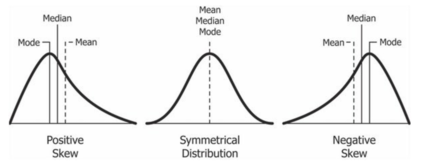
\includegraphics[scale=1.5]{SkewedData} \\
Data can also be bimodal, meaning it has two peaks \\
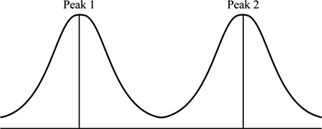
\includegraphics[scale=0.7]{Bimodal} \\

\section*{Measures of Central Tendency}
There are four measures of central tendency that we should be aware of:
\begin{itemize}
	\item Mode - The mode is the value that occurs most frequently. The distribution is uni-modal if there is only one mode. If two non-adjacent values occur mode frequently than the rest, the distribution is said to be bi-modal, even if the frequencies aren't the same. 
	\item Medial - It is the middle value. It is a good measure as it isn't skewed as much by outliers but most representative for symmetrical data. 
	\item Mean - Found by adding all the values together and dividing by the number of values. We use the symbol $\bar{x}$ to denote the mean. It is the best measure for skewed data but also representative for symmetrical data. It is affected by outliers. 
	\item Midrange - This is the average of the highest and lowest values. It is easy to calculate but only useful when the data is symmetrical and contains no outliers. 
\end{itemize}

\section*{Measures of Spread}
There are three measures of spread we need to know about which help us talk about how varied the data is.
\begin{itemize}
	\item Range - This is the highest subtract the lowest. Again this is not useful if we have any outliers.
	\item Interquartile Range - As seen before. We can also find the semi-interquartile range which is half the interquartile range.
	\item Standard Deviation - This we will learn about separately but is the most widely used measure of spread.   
\end{itemize}

\end{document}